\documentclass[conference]{IEEEtran}
\IEEEoverridecommandlockouts
\usepackage{cite}
\usepackage{amsmath,amssymb,amsfonts}
\usepackage{algorithmic}
\usepackage{graphicx}
\usepackage{textcomp}
\usepackage{xcolor}
\def\BibTeX{{\rm B\kern-.05em{\sc i\kern-.025em b}\kern-.08em
    T\kern-.1667em\lower.7ex\hbox{E}\kern-.125emX}}
\begin{document}


\title{Prediction of Train Ticket Price in Spain\\}
\author{\IEEEauthorblockN{1\textsuperscript{st} Dongzhan Xie}
\IEEEauthorblockA{\textit{University of Nottingham Ningbo China} \\
Ningbo, China \\
Email: scydx2@nottingham.edu.cn \\
Student ID: 20031862}
\and
\IEEEauthorblockN{2\textsuperscript{nd} Runxuan Bai}
\IEEEauthorblockA{\textit{University of Nottingham Ningbo China} \\
Ningbo, China \\
Email: scyrb1@nottingham.edu.cn\\
Student ID: 20030365}
\and
\IEEEauthorblockN{3\textsuperscript{rd} Shaolou Zhang}
\IEEEauthorblockA{\textit{University of Nottingham Ningbo China} \\
Ningbo, China \\
Email: scysz4@nottingham.edu.cn \\
Student ID: 20030263}
\and
\IEEEauthorblockN{4\textsuperscript{th} Zhangli Wang}
\IEEEauthorblockA{\textit{University of Nottingham Ningbo China} \\
Ningbo, China \\
Email: scyzw1@nottingham.edu.cn \\
Student ID: 20028336}
}
\maketitle


\begin{abstract}
This project aims to explore the price classification of Spanish train tickets using SPARK. The paper presents the data cleaning methods for various influencing factors and the classification methods of machine learning and proves that our model is optimized and able to predict fares with high accuracy. Various machine learning algorithms were used to predict the price of train tickets on the Spanish railway system based on different data types, such as different seats or classes of trains. Firstly, the relevant knowledge of the Spanish railway system is briefly introduced, and the data set cleaning methods by feature identification and deletion of missing and inaccurate data, and the data set with effective value is obtained by reducing unnecessary computation by random sampling method. Then the classification models used in this paper are introduced, including Logistic Regression Classification, One-vs-Rest base on Logistic Regression Classification, Bayes Classification, Decision Tree and Random Forest. The results show that the data factor of duration and  have the greatest influence on the train ticket price, and Logistic Regression Classification has the best learning effect, followed by Decision Tree. These two models have the best learning effect and the most accurate prediction result on the train ticket price. Another experimental result is that the discretization number of labels influences the fitting degree of algorithms non-monotonously.
\end{abstract}

\begin{IEEEkeywords}
big data, machine learning, spark, ticket price
\end{IEEEkeywords}

\section{Introduction}
At present, most timetable information systems provided by public transport services only convey information about travel time, ignoring other relevant criteria, in particular, the ticket cost \cite{b1}. Several studies have been conducted to explore the possibility of adding supplemental information beyond travel time and optimizing it for several criteria, including ticket costs. In order to optimize the overall fare, rapid numerical prediction of prices is needed. Rail companies, especially Renfe in Spain, use a very complex system of fares that do not necessarily correspond to the distance traveled. Many parameters determine the actual final fare, including but not limited to a number of complex factors such as departure and destination, departure date, duration, type of train, class of train, etc.
This paper focuses on the classification of train ticket prices, to understand the impact of different data characteristics, such as target, journey length, train class and date, on the classification of ticket prices. To figure out the impact, team members proposed a number of classification models suitable for big data requirements by cleaning data sets. A number of classification techniques were used in this project, including Logistic Regression Classification, Bayes Classification, One-vs-Rest, Random Forest and Decision Tree. Through these classification models, the train ticket costs can be predicted with maximum accuracy.
The paper relies heavily on the words most commonly used in the field of the Spanish railway system. Therefore, it is necessary to give a brief description of the Spanish railway system about the different passenger trains operating in Spain and their price structures. Take Spain's Renfe Railway Company as an example. The Spanish railway system can be divided into many types of trains, such as those mentioned in the study:

\begin{table}[ht]
\begin{center}
\caption{Spain's Train Type}
\begin{tabular}{|c|c|}
\hline
Train Type & Description \\ \hline
AVE & \begin{tabular}[c]{@{}c@{}}Short for Spain's high-speed trains, \\ which travel the fastest and cost the most.\end{tabular} \\ \hline
ALVIA & \begin{tabular}[c]{@{}c@{}}A high-speed train operated by Spain's \\ national rail service for long-distance travel.\end{tabular} \\ \hline
INTERCITY & Long distance trains, slower and cheaper. \\ \hline
MD-LD & \begin{tabular}[c]{@{}c@{}}Transfer from the mid-distance train to \\ the long-distance train.\end{tabular} \\ \hline
\end{tabular}
\end{center}
\end{table}

Spanish trains are also highly stratified. The AVE trains are divided into three classes of tickets for three different carriages: club (business), Preferente (first class) and Turista (second class). There are two types of second-class cars, the Turista (second-class) and the Turista Plus (comfortable second-class). The main difference between the three sizes of carriages is the service \cite{b2}. Different types and different classes of the train to a large extent on the impact of the train ticket cost.

In the project, the only used data set is an open-source data set about the Spanish railway fare from Kaggle, the data set creator is David Adrián Cañones Castellano \cite{b3}. Sincerely appreciate for their sharing spirit. In this data set, the number of rows is 38.8 million, after data cleaning, 8 million rows (20.62\%) were selected for the next modelling. Several zoom ratios had been tried and tested, then the ratio of 0.05 was finally selected. In the modeling period, the train and test subsets were split with 70\% and 30\%. These basis and rationality are elaborated in the following parts.

Faced with the large amount of data set, we did a lot of preparation work for data cleaning in the early stage. Through feature identification and deletion of missing and inaccurate values, we obtained a featured data set. The data set is shrunk by random sampling to reduce unnecessary computation. After data cleaning, we put the data set into a variety of classification models, with the proof that the accuracy of the machine learning algorithm can converge with the size of sampling. Five feasible machine learning algorithms are deployed and hyper-parameters are optimized. We also analyzed the results for parameter tuning and other factors.

\section{Literature review}
\subsection{Predicting Germany railway fares in multiple machine learning methods}
In recent years, machine learning on the mathematical models of railway fares had expanded many different approaches. Hirschmann \cite{b1} studied and evaluated four different types of machine learning methods for predicting German railway fares, which are Decision Trees, Support Vector Machines, Linear Regression based algorithms and Artificial Neural Networks. In his paper, the whole process has expatiated from data preparation to model evaluation, the transformation from continuous values to discrete values (labels) is referred to in our research. According to Hirschmann’s result, the Decision Tree learner cubist from Quinlan \cite{b4} performed best but Linear Regression \cite{b5} \cite{b6} got a relatively inaccurate result. This is probably because Hirschmann used a data set from the German railway before 2008, until then, Deutsche Bahn (German Railways) priced railway tickets mainly dependent on the traveling distance. However, the traveling distance is a relatively fixed factor unlike traveling duration, which might not be affected by vehicle type and stopping time. In our research of predicting Spanish railway fares, there are multiple conclusive factors to determine ticket prices, such as vehicle class and preferential policies. For evaluating the prediction result impact of irrelevant variables on different pricing factors under the same algorithm, both the Decision Tree algorithm and the Linear Regression based algorithms (Logistic Regression and One-Versus-Rest Logistic Regression) were implemented. 

\subsection{Machine learning and classification algorithms on big data using Apache Spark}
Apache Spark unifies programming model and engine for big data applications \cite{b7}, the generated intermediate and the final output results from Spark workflows can be stored in memory for improving the efficiency of data computing which is called Memory Computing \cite{b8}. In addition, another advantage is that Spark revolves around the concept of Resilient Distributed data set (RDD) can be used to achieve parallel programming models such as iterative algorithms and SQL queries Therefore, Spark is suited for Machine Learning. Samar, Ghazi and Arafat applied three classification algorithms included Logistic Regression, Naive Bayes and Support Vector Machine under Apache Spark to classify large-scale sentiment data in online reviews \cite{b9}, after data preprocessing, they extracted the text into labels for Spark MLlib classifiers to read, this method applies to the stations in our database. Yulong studied and improved the efficiency of classical Random Forest algorithms on large database backgrounds \cite{b10}, the formulas of meta-classifier were tested during our parameter optimization process. Additionally, an evaluation of the MLlib library in Spark classification algorithms for predicting the customer’s behavior of the Spanish Standard Bank showed that the Naïve Bayes classifier performs more efficiently on precision, recall and f-measure than the Support Vector Machine classifiers \cite{b11}. Their methods of processing and classifying the huge data set for adapting Spark were referred to in this research. In this project, these algorithms are implemented, after that, five applicable models for the given data set were selected for further optimization.

\subsection{Adapting One-vs-Rest strategy in the multi-class classification problem}
One-vs-Rest (OvR) is a heuristic method that uses the classical binary classification algorithms and updates the strategy to multi-class classification, OvR strategy is usually used for naturally numerical classification of membership probability or scoring algorithms, such as Perceptron and Logistic Regression \cite{b12}. According to an application of Logistic Regression based on OvR strategy \cite{b13}, in order to convert a binary classifier to a multi-class classifier by using the OvR, the first step is during the testing process. Train a set of binary classifiers and calibrate one of them with the positive prediction result. At the same time, set those remaining categories as anti-class prediction results, so the classifiers should contain one positive and the rest are anti-class. The second step, pass all the data through three (or more) identifiable binary classifiers, after that, the final prediction result should be positive. Subsequently, if the prediction of multiple classifiers is also positive, the determining factor should be reconsidered as the prediction confidence, and select the category with the highest prediction confidence as the final category \cite{b13}. For the past few years, there are plenty of ways to optimize the OvR strategy, one approach is to feed two experts at the first step, one is the true expert as the usual OvR, the other one is the misclassified expert with the highest confidence, each expert will be given two subsets of the labeled instances for training and further updating \cite{b14}, this approach relieves the problem of imbalanced training data.

\subsection{Approaches of data preprocessing}
Rahm and Do studied the approaches for improving data quality, as the result, consolidate different data representation and eliminate duplicate information is an indispensable process \cite{b15}. Acuna, Rodriguez, Liu and Lei believes that missing more than 15\% of the data is missing in a variable may severely impact any kind of data interpretation \cite{b16}\cite{b17}, and a study showed that the performance of Decision Tree classifier decreases sharply as the missing percentage increases from 10\% \cite{b18}. Therefore, the preprocessing process to data set with numerous missing values is necessary. Additionally, in our project, a part of raw continuous labels must be transformed into discrete labels. It is possible that discretization may potentially result in the loss of information. It is possible that slight discretization may potentially result in severe loss of information. To research the consequences of this phenomenon, researchers compared several discretization methods for Bayesian networks (BNs), including interval, quantile, and moment matching \cite{b19}. The result demonstrated that if the data set is large and the model is simple, the goodness of fit can mitigate the impact of types of discretization method. In our project, with the type of discretization fixed as invariable, we study the impact of the quantity of discretization on the fitting of machine learning algorithms.

\section{Methodology}
\subsection{Data Preparation}
In the machine learning field, data quality plays a critical role in training and testing models. Lack of data quality manifests in several forms, including missing data, inaccurate values, duplication, and inconsistency\cite{b20}. A data clean procedure before the training of machine learning algorithms aims to tackle the lack of data quality.
\subsubsection{Feature Identification and Selection}
In this subsection, we aim to identify and select useful features for machine learning algorithms to predict ticket price. Compared to the raw data set, the “company” column is dropped due that it has only one unique attribute so that it does not influence the prediction. Columns “insert\_date” and “id” representing the date of insertion row to the data set and id of the row respectively are dropped due that their have no relevance to the prediction result. Besides, the feature “seats” representing the vacancy seats are dropped. The reason is that if this feature is reserved, the continuity of the time series data set is destroyed due that majority of rows with missing class values must be deleted for machine learning. According to pricing rules specified in the official website of Renfe\cite{b21}, the ratio of discount is clearly specified. Hence, we can shrink  the “fare” feature, which represents discounted ticket types, by only selecting the rows with the “flexible” value of “fare”.
\begin{table}[ht]
\begin{center}
\caption{Feature Descriptions}
\begin{tabular}{|l|l|}
\hline
\multicolumn{1}{|c|}{\textbf{Feature Name}} & \multicolumn{1}{c|}{\textbf{Description}} \\ \hline
origin                                      & departure station                         \\ \hline
destination                                 & destination station                       \\ \hline
departure                                   & departure date                            \\ \hline
arrival                                     & arrival date                              \\ \hline
duration                                    & total journey duration                    \\ \hline
vehicle\_type                               & train type of Renfe                       \\ \hline
vehicle\_class                              & train class of Renfe                      \\ \hline
price                                       & ticket price in euros                     \\ \hline
\end{tabular}

\end{center}
\end{table}
\subsubsection{Missing and Inaccurate Values}
After feature selection, few instances of missing and inaccurate values have remained. For this problem, we take a measurement to drop the rows that any feature has missing value with a SQL query in Spark. Besides, rows that price is zero value are removed simply because that it is unrealistic.
\subsubsection{Sampling}
Since in this project, machine learning algorithms are trained in local mode in Spark, a sampling process should be executed for the data set to reduce the amount of computation. For practice, we performed a random sampling with a relatively large scale to shrink the data considering at the same time the data instances should be sufficient. In a future experiment (table), it is proved that the accuracies of machine learning algorithms can converge with the scale of sampling.
\subsubsection{Data Transformation}
In this subsection, we plan to transform the format of the data set to conform with the restrictions of classification algorithms in Spark. In the first place, we transform the string-typed attributes to integer-typed labels. For continuous attributes, we implemented quantile discretization, which is not affected by non-linear transformations\cite{b22}. According to Gupta, Thakur\cite{b23}, a one-hot encoding is implemented at the end of data transformation for compatibility with Spark machine learning libraries. When this step is completed, the data set can be input into a classification algorithm in Spark.
\subsubsection{Attribute Correlation}
We performed preliminary data analysis on the processed data set to validate it. According to MA Hall\cite{b24}, a central hypothesis of machine learning is that ideal features in the data set should have a high correlation with the label, but uncorrelated to each other. In our project, in the correlation matrix of selected features, most Pearson correlation coefficients between pairs of features are less than weak correlation. This means that the data set is valid for machine learning.
\begin{figure}[ht]
\centering
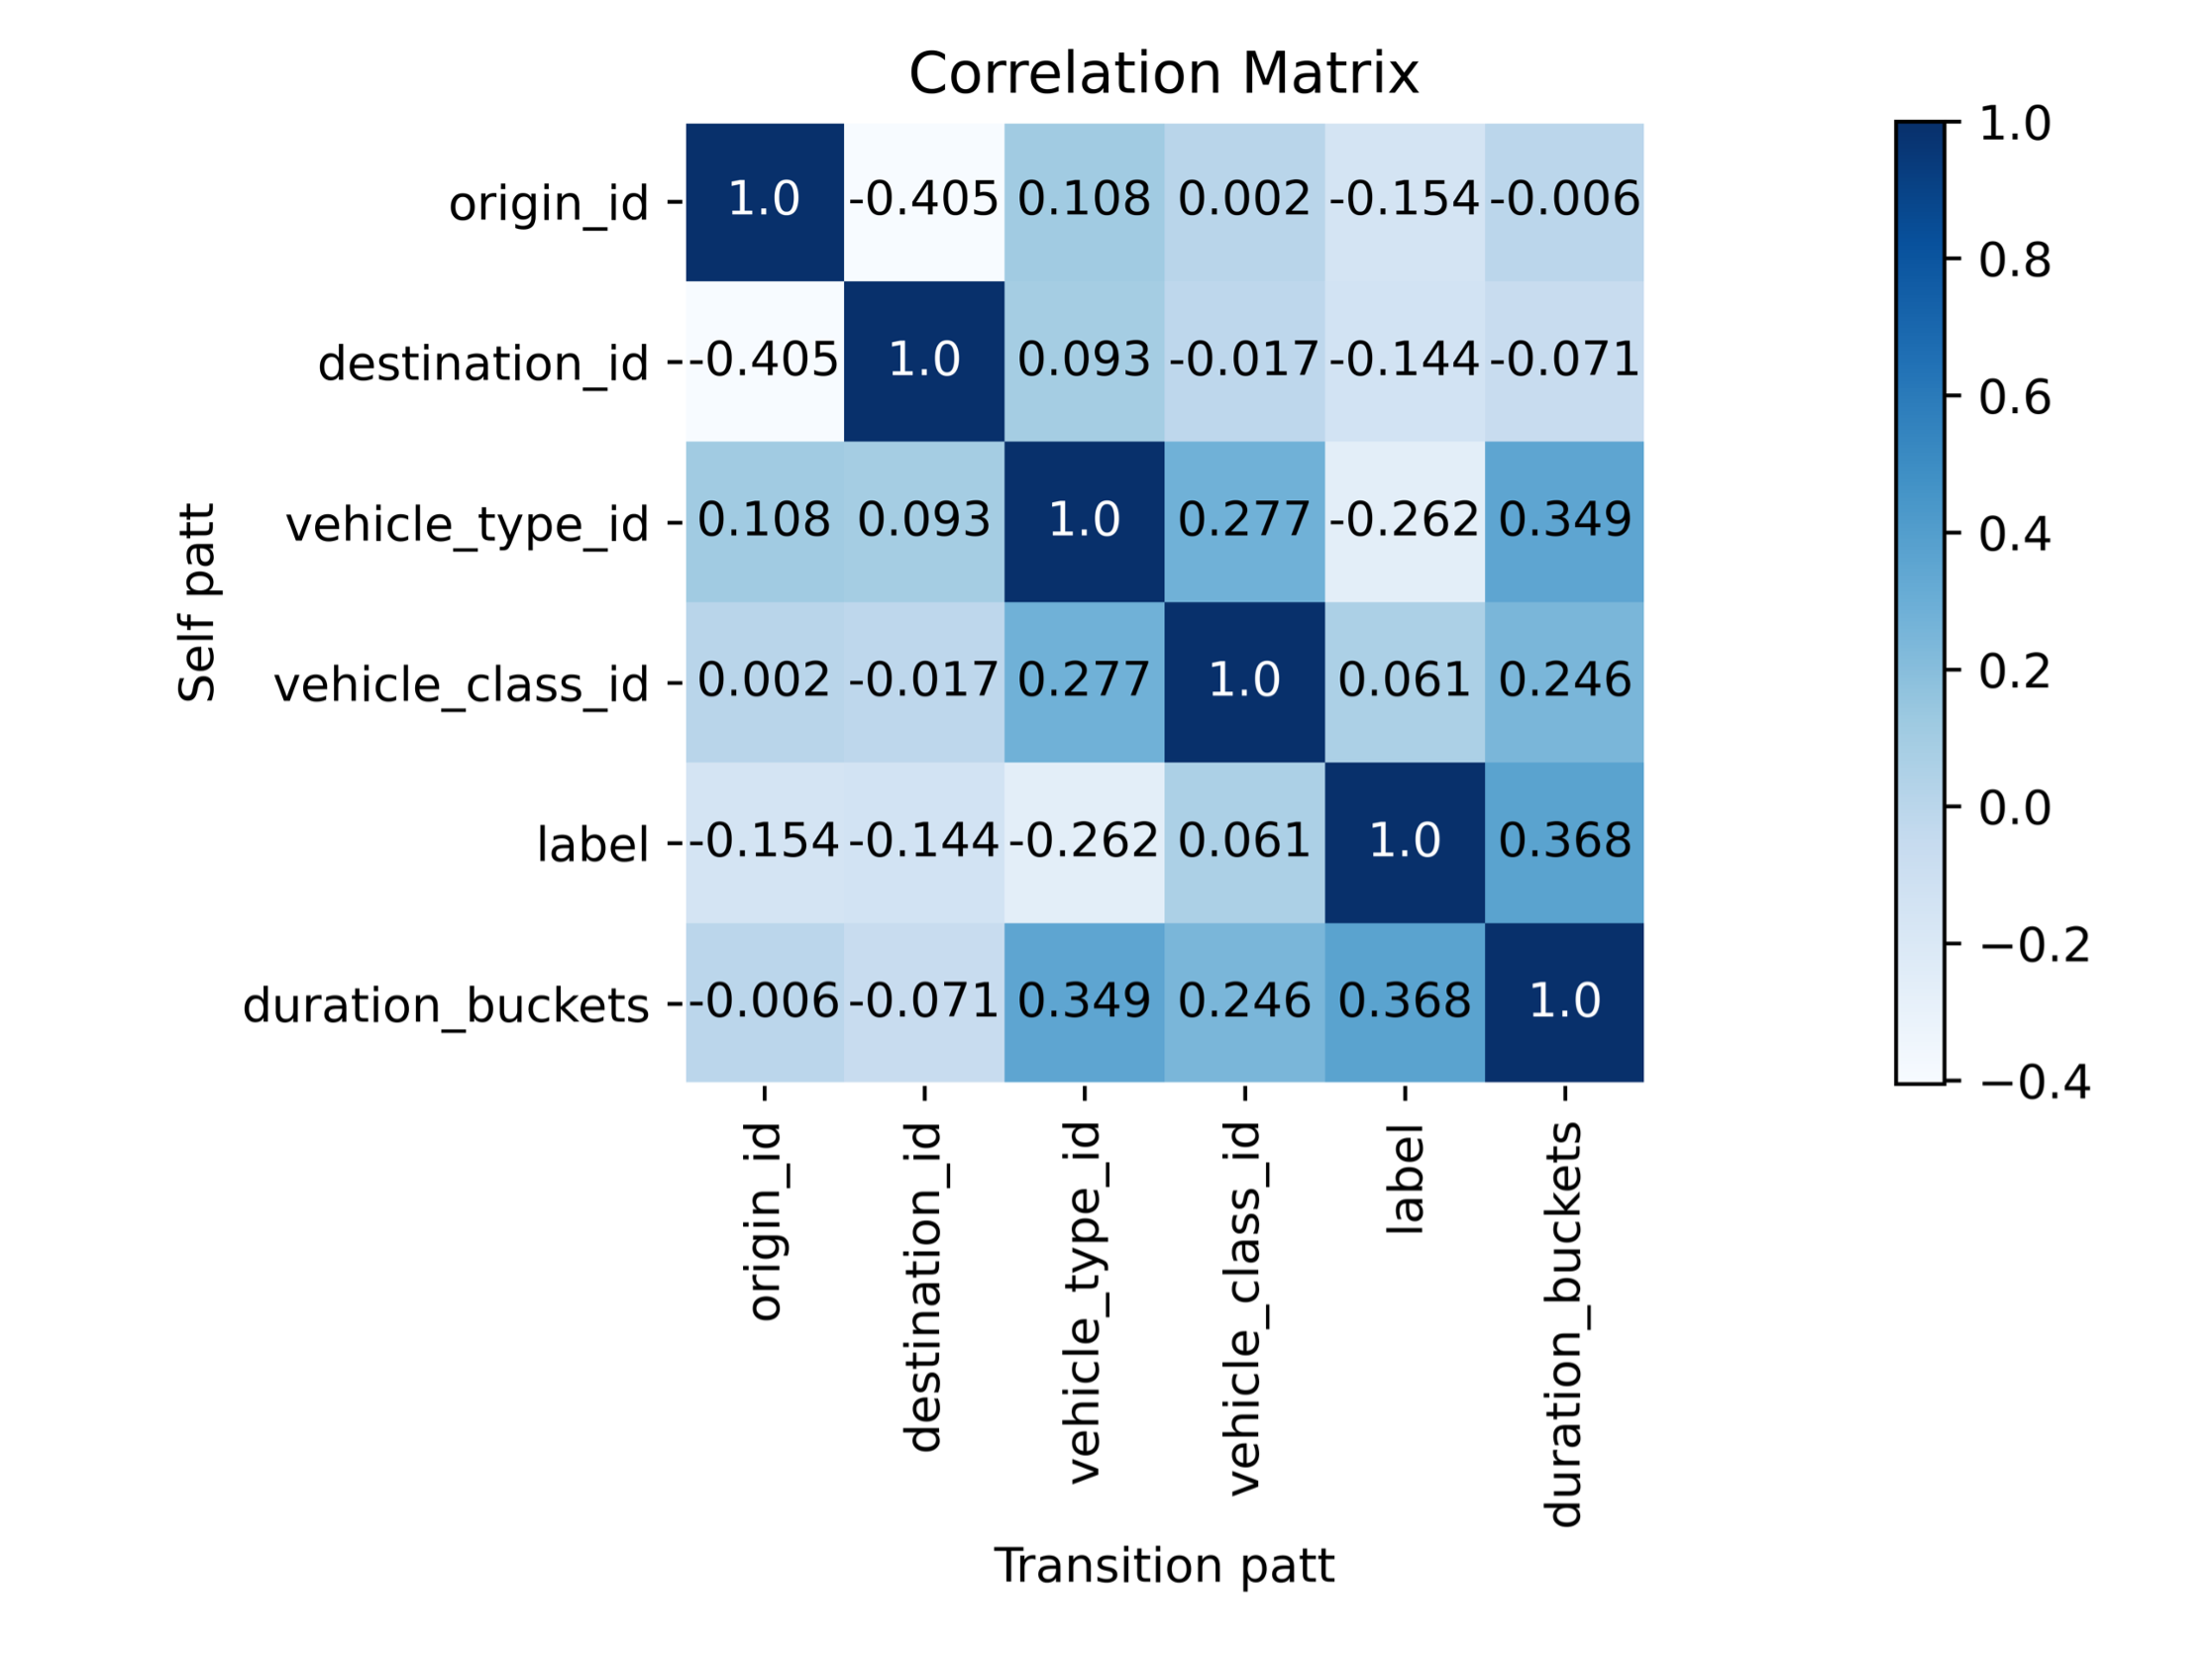
\includegraphics[width=6cm]{01.png}
\caption{Correlation Matrix of Selected Features}
\end{figure}

\subsection{Machine Learning Model}
To achieve the prediction of train fares in Spain, we chose to use MLlib, a distributed machine learning library on the Spark open-source platform, to establish a machine learning classification model suitable for big data. Benefiting from Spark's optimization for iterative computation and data parallelism, MLlib shows excellent performance in processing large-scale machine learning algorithms\cite{b25}. 
\subsubsection{Flow of Machine Learning Model Establishment}
Firstly we need to convert the CSV file generated during the data pre-processing phase into the DataFrame  which is required for the machine learning algorithm. DataFrame supports operations using SQL statements, allowing for more convenient adjustment of data. Spark MLlib provides a method to convert CSV files to DataFrame after version 2.0 \cite{b26}. Then we randomly split the entire DataFrame into a training set (70\%) and a test set (30\%) using the randomSplit method in MLlib. Through the MLlib, we established five different machine learning classification models including Logistic Regression, Decision Tree, Random Forest, Bayes classification and the "One-vs-Rest" model based on Logistic Regression. The model was trained by calling the model-owned method fit(), where the input is the training set. Once training is complete, we will save the currently trained model for future analysis and manipulation. In order to find the most suitable model, we need to perform an evaluation for each model. Accuracy is one of the most important factors in measuring the merit of a model. As the classification of price labels is not binary, we need to use the MulticlassClassificationEvaluator in MLlib to evaluate the model. The prediction accuracy of the model would be obtained by setting the labelCol, predictionCol and metricName of the MulticlassClassificationEvaluator.
\begin{figure}[ht]
\centering
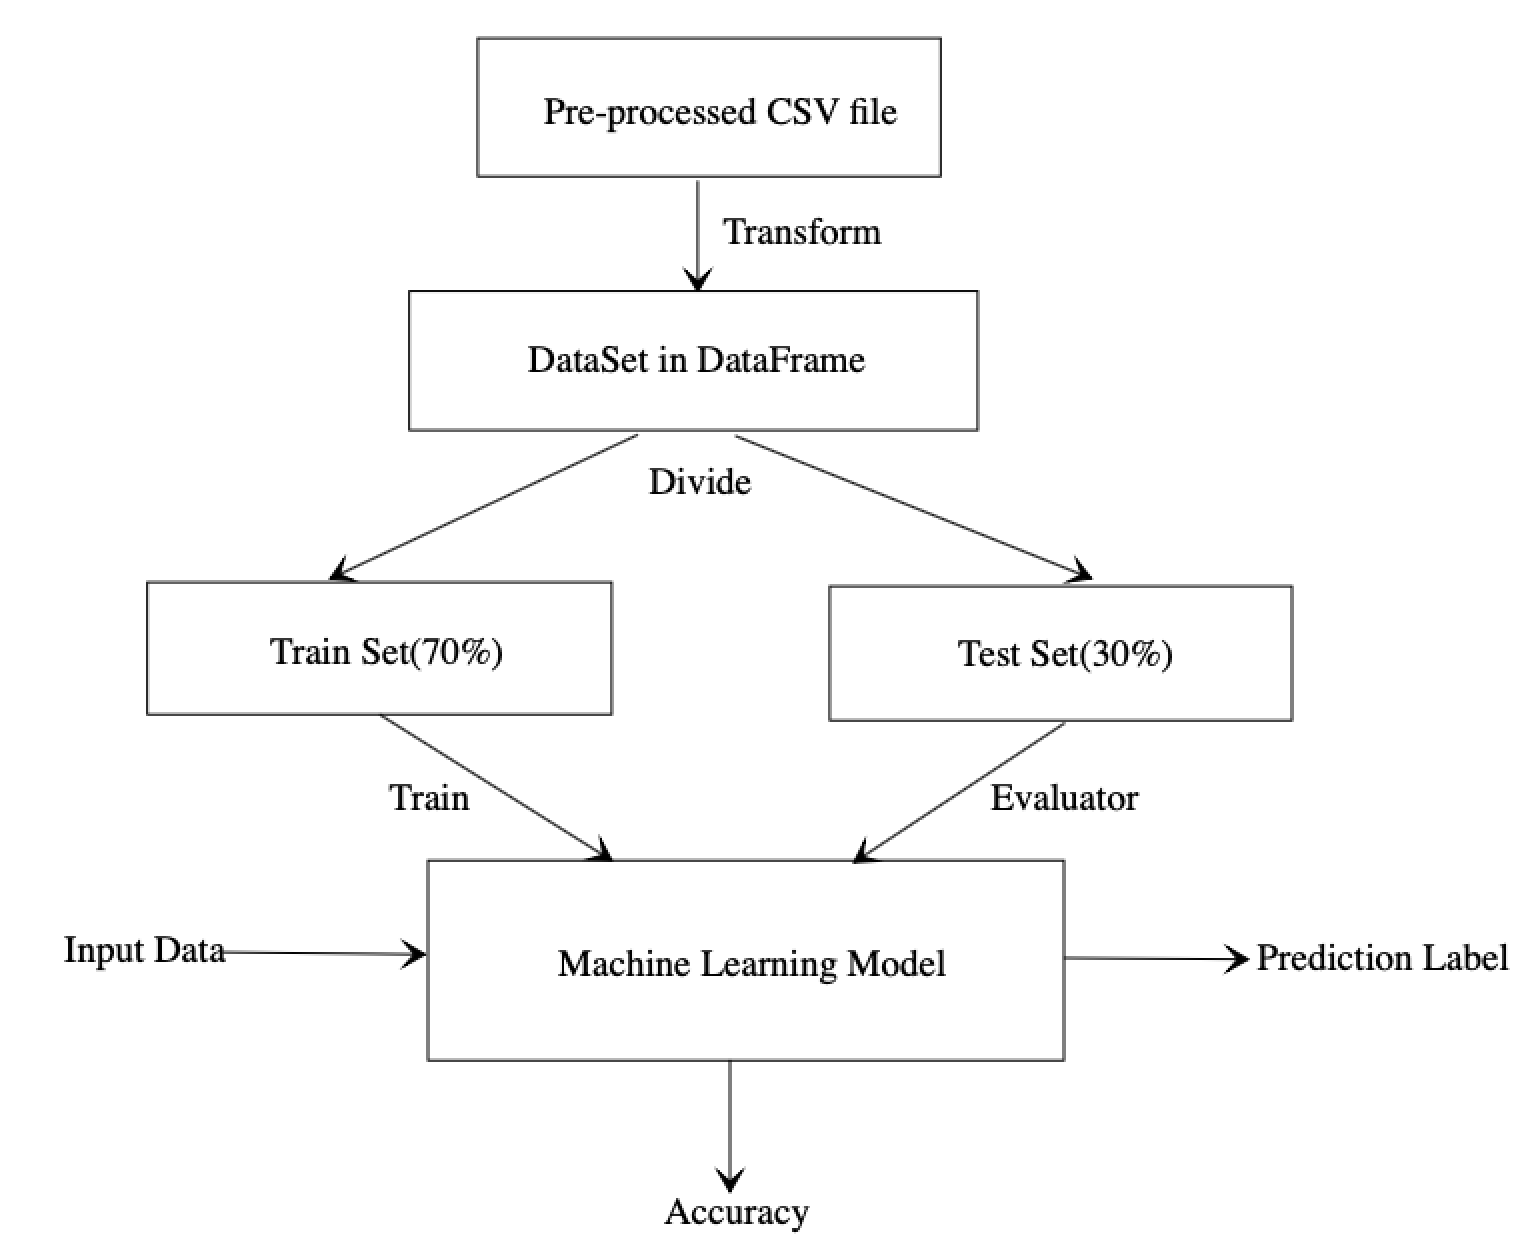
\includegraphics[width=6cm]{02.png}
\caption{The Flow of Machine Learning Model Establishment}
\end{figure}
\subsubsection{Optimization of the machine learning model}
In order to improve the accuracy and training speed of the model, we need to optimize the machine learning model. The easiest and most effective way to achieve it is to tune the parameters of the machine learning algorithm based on your own data. Although we were unable to directly find the exact practical meaning of the corresponding parameters due to the complexity of relationships between their effects. Manual tuning of machine learning parameters by trial-and-error methods would take a significant amount of time\cite{b27}. However, after numerous experiments and attempts, we eventually optimized the performance of a portion of the machine learning model. Specific experimental data to optimize the performance of the machine learning models will be presented in the RESULT AND DISCUSSION section.



\section{Result and discussion}
\subsection{Results of machine learning model optimization}
\subsubsection{Logistic Regression model}
In the MLlib library, the developer is allowed to regularize the model by tuning the regParam and elasticNetParam parameters of the Logistic Regression model. Regularization adds penalty coefficients to the regression equation avoiding the decrease in accuracy due to overfitting\cite{b28}. Default values of regParam and elasticNetParam in the Logistic Regression model are both 0, indicating that no regularization is performed on the regression equation without parameter tuning. The higher the value of regParam, the stronger is the effect of the penalty coefficient on the regression equation. MLlib provides an elasticNet API, allowing developers to change the type of regularization penalty coefficient by adjusting the elasticNetParam. The range of elasticNetParam is from 0 to 1. When elasticNetParam is 0, the Linear Regression model is the Lasso model, and when elasticNetParam is 1, the Linear Regression model is changed into Ridge Regression model \cite{b29}. 

We experimented with a Logistic Regression model at maxIter = 100, data scaling = 0.15, price label = 8. The accuracy of the model is shown in the table below:
\begin{table}[ht]
\begin{center}
\caption{Accuracy of Logistic Regression model \\under different parameters}
\begin{tabular}{|l|l|l|l|l|}
\hline
                                                                & \begin{tabular}[c]{@{}l@{}}regParam\\ = 0\end{tabular} & \begin{tabular}[c]{@{}l@{}}regParam\\ = 0.005\end{tabular} & \begin{tabular}[c]{@{}l@{}}regParam\\ = 0.01\end{tabular} & \begin{tabular}[c]{@{}l@{}}regParam\\ = 0.1\end{tabular} \\ \hline
\begin{tabular}[c]{@{}l@{}}elasticNetParam\\ = 0\end{tabular}   & 0.974                                                  & 0.951                                                      & 0.944                                                     & 0.801                                                    \\ \hline
\begin{tabular}[c]{@{}l@{}}elasticNetParam\\ = 0.5\end{tabular} & 0.974                                                  & 0.935                                                      & 0.922                                                     & 0.798                                                    \\ \hline
\begin{tabular}[c]{@{}l@{}}elasticNetParam\\ = 1.0\end{tabular} & 0.974                                                  & 0.943                                                      & 0.890                                                     & 0.796                                                    \\ \hline
\end{tabular}
\end{center}
\end{table}

The table shows that, with the same elasticNetParam, as the parameter regParam increases, the influence of penalty coefficient on the Logistic Regression model increases and the accuracy of the model decreases. In the case of the same regParam, as the parameter elasticNetParam increases, the effect of Ridge regression model on the Regression model strengthens, the effect of Lasso model on the Regression model weakens and the accuracy of the model decreases gradually. We can conclude that since our data set is well-suited for model training, our model has an excellent fitting to the data and there is basically no overfitting problem. Therefore, using regularization for the regression equation will reduce the accuracy of the model. In summary, our recommended parameters for the Logistic Regression model are: regParam = 0, elasticNetParam = 0. 

\subsubsection{Random Forest Classification Model}
In the Random Forest classification model, the fitting degree of the model can be adjusted by tuning maxDepth and numTrees parameters, where the default value of maxDepth is 5 and the default value of numTrees is 20. A larger value of maxDepth means a more complex model and a higher degree of model fit. High maxDepth may lead to overfitting of the model. A larger value of numTrees also means a higher degree of model fit. However, since the Random Forest algorithm uses a random selection of features, the generalization ability of the model will be reduced with too many trees \cite{b30}. 

We experimented with a Random Forest Classification Model at data scaling = 0.15, price label = 8. The accuracy of the model is shown in the table below:
\begin{table}[ht]
\begin{center}
\caption{Accuracy of Random Forest model \\under different parameters}
\resizebox{.95\columnwidth}{!}{
\begin{tabular}{|l|l|l|l|l|l|}
\hline
                                                        & \begin{tabular}[c]{@{}l@{}}maxDepth\\ = 3\end{tabular} & \begin{tabular}[c]{@{}l@{}}maxDepth\\ = 5\end{tabular} & \begin{tabular}[c]{@{}l@{}}maxDepth\\ = 10\end{tabular} & \begin{tabular}[c]{@{}l@{}}maxDepth\\ = 20\end{tabular} & \begin{tabular}[c]{@{}l@{}}maxDepth\\ = 40\end{tabular} \\ \hline
\begin{tabular}[c]{@{}l@{}}numTrees\\ = 15\end{tabular} & 0.647                                                  & 0.787                                                  & 0.906                                                   & 0.985                                                   & 0.982                                                   \\ \hline
\begin{tabular}[c]{@{}l@{}}numTrees\\ = 20\end{tabular} & 0.667                                                  & 0.812                                                  & 0.906                                                   & 0.984                                                   & 0.987                                                   \\ \hline
\begin{tabular}[c]{@{}l@{}}numTrees\\ = 25\end{tabular} & 0.654                                                  & 0.810                                                  & 0.911                                                   & 0.990                                                   & 0.985                                                   \\ \hline
\end{tabular}
}
\end{center}
\end{table}
The table shows that when maxDepth is less than 20, the accuracy of the model rises as maxDepth increases; when maxDepth is greater than 20, the accuracy of the model does not rise even if maxDepth continues to increase. There is no intuitive pattern in the effect of changing numTrees on the accuracy rate. This situation is probably caused by the random selection strategy in the random forest algorithm. We can conclude that at lower maxDepths including default maxDepth, our model is under fitted to the data, increasing the maxDepth of the model will result in a significant improvement in accuracy. When the maxDepth is greater than 20, the model is already fitted, and increasing the maxDepth will not only not increase the accuracy of the model, but also raise the computational complexity. In summary, our recommended parameters for the Random Forest Classification Model are: maxDepth = 20, numTrees = 20. 

\subsection{Results of influence of Fraction}
\begin{table}[ht]
\begin{center}
\caption{Accuracy of Logistic Regression with different fraction of data shrinking with discretization number valued 10}
\begin{tabular}{|l|l|}
\hline
Fraction of Data Shrinking & Accuracy of Logistic Regression \\ \hline
0.05                       & 0.891515                        \\ \hline
0.5                        & 0.890344                        \\ \hline
\end{tabular}
\end{center}
\end{table}

According to the diagram, when the output class is discretized to 10 buckets, the impact of the shrinking fraction on the machine learning results is insignificant. For instance, when the shrinking fraction of the raw data set is set to 0.05, the training accuracy of the machine learning algorithms is identical as ones with the fraction 0.5. For analysis, the reason can be accounted as the raw data set is large and the models can be simple. Therefore, the models can be fitted with a small scale of data set.

\subsection{Result of influence of Discretization Number}
\begin{figure}[ht] 
\centering
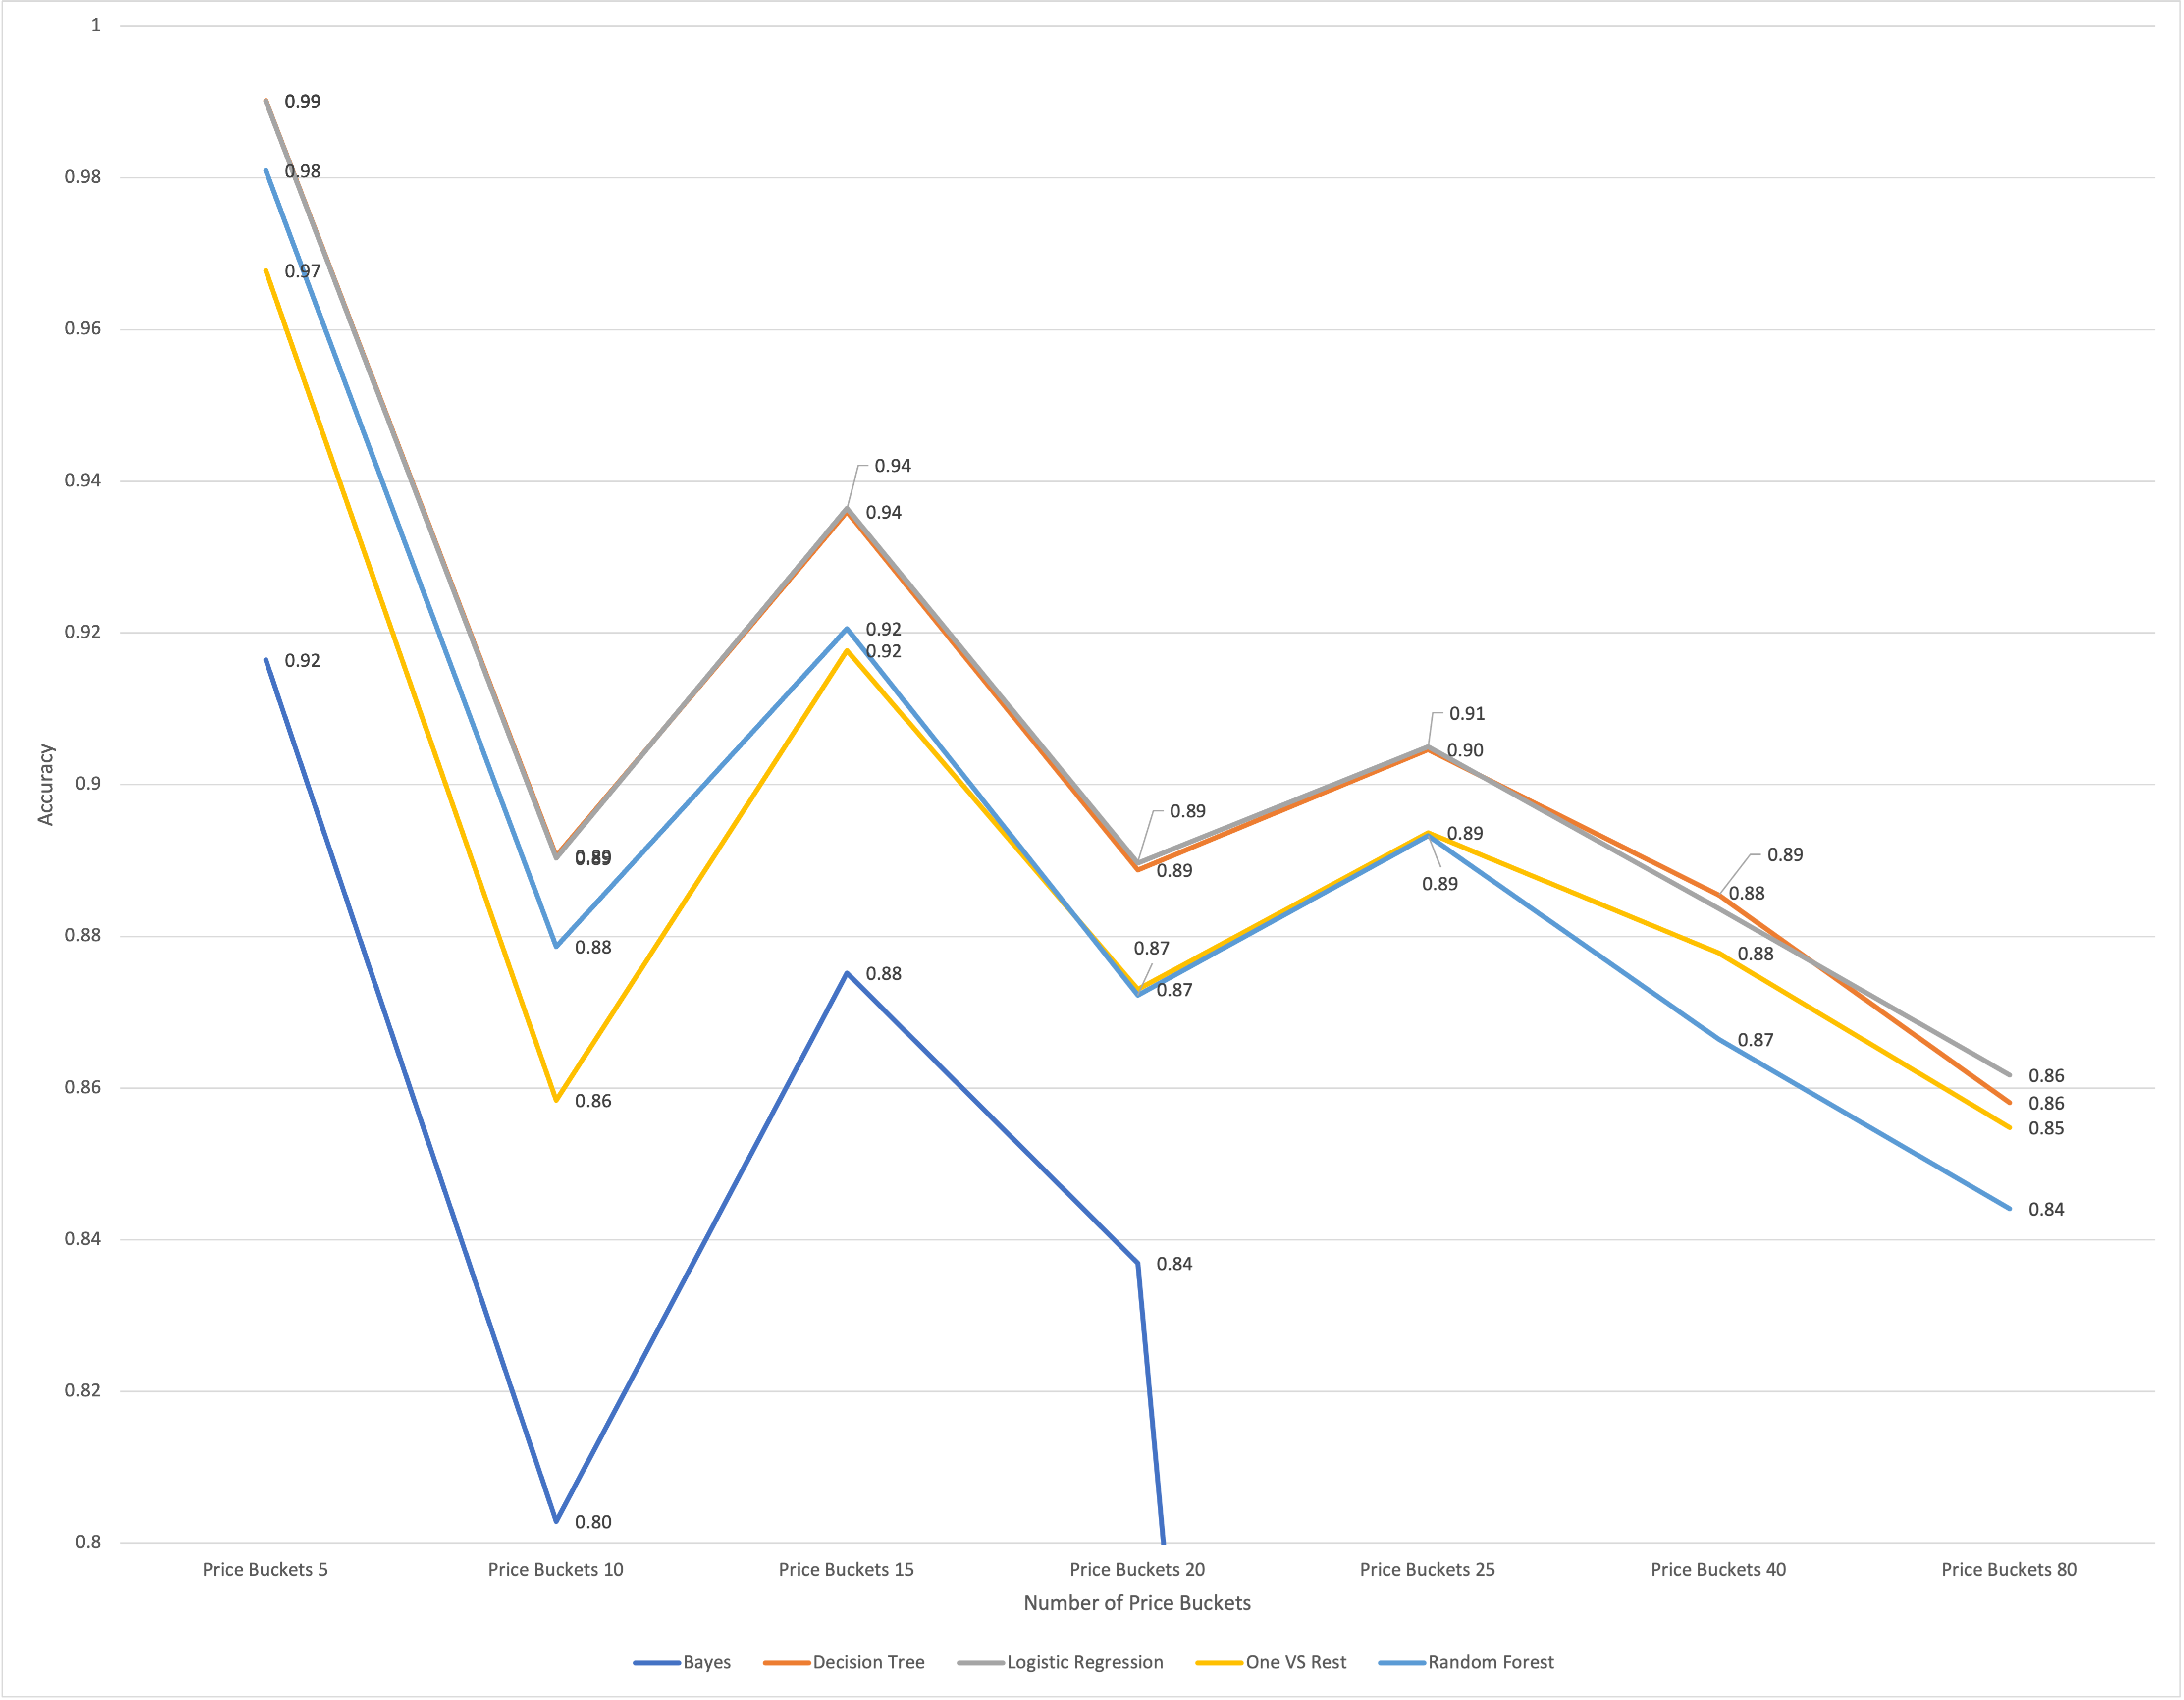
\includegraphics[width=8cm]{03.png}
\caption{Accuracy of machine learning algorithms with different discretization number with fraction valued 0.05}
\end{figure}

In our hypothesis, the larger number of labels can result in greater complexity of constructing models. Hence, the accuracies of algorithms decrease as the number of discretization increases. As the diagram demonstrates, the amount of discretization of the label can influence the accuracies of machine learning algorithms. We researched the variable discretization number from 5 to 80, the demonstrated figure presents a non-monotonous curve which is in contrast to the hypothesis. In our analysis, when the discretization number is excessively small, the lacking complexity of the data set can result in that the algorithms are trained too uncomplicated that accuracy measurement is trivial. When the discretization value is at a certain interval, the instances of feature vectors may be most representative of their assigned labels. Therefore, the two factors, the complexity of model and discretization error, maybe balanced for an optimized result. When the discretization value is excessively large, the model can be excessively complex thus the accuracy rates may decrease. Similar situations have appeared in a related study\cite{b30}.

Since when the discretization number is excessively small, the accuracy rates of machine learning algorithms may not have a reference value as the data set can be too uncomplex. The optimized and valuable accuracy in this research is reached when the class is discretized into 15 number of buckets for the Logistic Regression Algorithm. Finally, the accuracy is shown in table TODO with hyper-parameters.

\begin{table}[ht]
\begin{center}
\caption{optimized accuracy of Logistic Regression with hyper-parameters}
\begin{tabular}{|l|l|l|}
\hline
\begin{tabular}[c]{@{}l@{}}Discretization\\ Number\end{tabular} & \begin{tabular}[c]{@{}l@{}}Fraction of \\ Data Shrinking\end{tabular} & \begin{tabular}[c]{@{}l@{}}Accuracy of \\ Logistic Regression\end{tabular} \\ \hline
15                                                              & 0.05                                                                  & 0.936415                                                                   \\ \hline
\end{tabular}
\end{center}
\end{table}

\subsection{Comparison with the results of a related study}
Combined with Hirschmann’s result, it is obvious to find that the Decision Tree classifier (Cubist Tree is an expanded branch) is highly efficient in analyzing railway fares, a possible assumption is the pricing strategy among tariff systems is similar to the tree structure. For example, there is always a fixed top price, the original price for the most comfortable seat with the same vehicle class. Then, types of seat (preferent or common) offer different her fixed discounts. The other factors may be multilayered or parallel. This is highly compatible with the data structure of the Decision Tree classification. On the other hand, Hirschmann’s Linear Regression classifier on the German railway data set performed an average level, but the Linear Regression based classifier, Logistic Regression performed best on the Spanish data set. The reason might be the principle influencing factor is different. The German railway adopted the relatively steady traveling distance as the main basis whereas the Spanish adopted traveling duration which could be affected by multivariant factors such as traveling distance, vehicle type and vehicle class.
\begin{figure}[ht]
\centering
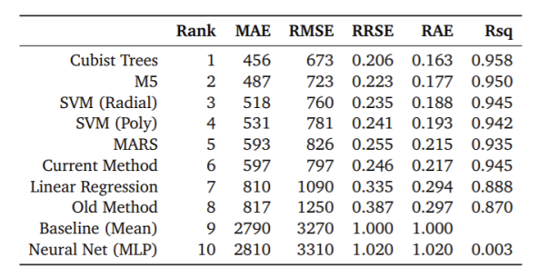
\includegraphics[width=7cm]{04.png}
\caption{The accuracy ranking of different classifiers in Hirschmann’s result.\cite{b1}}
\end{figure}
\section{Conclusion}
The paper elaborates on our project on predicting Spanish railway fares. Within this thesis, we have presented the methodologies of the cleaning of big data, related data presentation and transformation. Necessary theoretical demonstrations are referred to prove the necessity and rationality of data processing and parameter adjusting. Moreover, the tunning process and final results of the five implemented classification methods are compared. In these classifiers, the Logistic Regression gets the best accuracy of 93.64\% with set the discretization number as 15, the fraction of data shirking as 0.05, then the Decision Tree takes the second ranking with a slight decline within 1\%. The third place and the fourth place are Random Forest and One-vs-Rest, their performance is also efficient, the accuracy reduced within 2\% compared with Logistic Regression. At the last place of the ranking, the accuracy of the Bayes reduced to 87.52\%. At the beginning stage, we expected the Decision Tree could perform the highest accuracy over 90\%, and we successfully achieved the goal. The specific analysis for the result is given in the paper. Besides, a discovery in our project shows the shrinking fraction over 0.05 lead to an insignificant impact on the huge data set while performing machine learning, but the discretization number has a significantly intuitive effect on the results, the analysis is given in the result part. In terms of the results on the test subset, the extremely high accuracy illustrates that the pricing strategy of the Spanish railway is stable and reasonable. On the other hand, Spark’s ability on processing big data is efficient, the classifiers are powerful enough to interpret the different representations of data and processing parallel computing.
\begin{thebibliography}{00}
\bibitem{b1} F. Hirschmann, “Machine learning for the prediction of railway fares,” 2013.
\bibitem{b2} "Spain Rail", 2021. [Online]. Available: https://spainrail.com/zh. [Accessed: 03- May- 2021].
\bibitem{b3} "Spanish Rail Tickets Pricing - Renfe", Kaggle.com, 2020. [Online]. Available: https://www.kaggle.com/thegurusteam/spanish-high-speed-rail-system-ticket-pricing. [Accessed: 20- Mar- 2021].
\bibitem{b4} Quinlan, J.R., “Induction of Decision Trees”, Machine Learning, 1986, pp. 81–106, doi: 10.1007/BF00116251
\bibitem{b5} Bishop, C.M., Neural Networks for Pattern Recognition. New York, NY, USA: Oxford University Press, Inc. 1995.
\bibitem{b6} Witten, L. H., Frank, E, and Hall, M. Data Mining: Practical Machine Learning Tools and Techniques. 3rd ed. San Francisco, CA, USA: Morgan Kaufmann, 2011, pp. 11, 19, 20, 34
\bibitem{b7} Communications of the ACM, https://dl.acm.org/doi/fullHtml/10.1145/ 2934664
\bibitem{b8} J. Fu, J. Sun and K. Wang, "SPARK – A Big Data Processing Platform for Machine Learning," 2016 International Conference on Industrial Informatics - Computing Technology, Intelligent Technology, Industrial Information Integration (ICIICII), 2016, pp. 48-51, doi: 10.1109/ICIICII.2016.0023.
\bibitem{b9} S. Al-Saqqa, G. Al-Naymat and A. Awajan, "A Large-Scale Sentiment Data Classification for Online Reviews Under Apache Spark", Procedia Computer Science, no. 141, pp. 183-189, 2018.
\bibitem{b10} Y. Xu, "Research and implementation of improved random forest algorithm based on Spark," 2017 IEEE 2nd International Conference on Big Data Analysis (ICBDA), 2017, pp. 499-503, doi: 10.1109/ICBDA.2017.8078683.
\bibitem{b11} W. Etaiwi, M. Biltawi and G. Naymat, "Evaluation of classification algorithms for banking customer’s behavior under Apache Spark Data Processing System", Procedia Computer Science, vol. 113, 2017, pp. 559-564, doi: 10.1016/j.procs.2017.08.280
\bibitem{b12} F. Perronnin, Z. Akata, Z. Harchaoui and C. Schmid, "Towards good practice in large-scale learning for image classification," 2012 IEEE Conference on Computer Vision and Pattern Recognition, 2012, pp. 3482-3489, doi: 10.1109/CVPR.2012.6248090.
\bibitem{b13} Y. Sun, Z. Zhang, Z. Yang and D. Li, "Application of Logistic Regression with Fixed Memory Step Gradient Descent Method in Multi-Class Classification Problem," 2019 6th International Conference on Systems and Informatics (ICSAI), 2019, pp. 516-521, doi: 10.1109/ICSAI48974.2019.9010220.
\bibitem{b14} S. Hashemi, Y. Yang, Z. Mirzamomen and M. Kangavari, "Adapted One-versus-All Decision Trees for Data Stream Classification," in IEEE Transactions on Knowledge and Data Engineering, vol. 21, no. 5, pp. 624-637, May 2009, doi: 10.1109/TKDE.2008.181.
\bibitem{b15} E. Rahm and H. Do, "Data Cleaning: Problems and Current Approaches", IEEE Data Engineering Bulletin, vol. 23, p. 5, 2000. Available: https://dblp.org/db/journals/debu/debu23.html. [Accessed 17 April 2021].
\bibitem{b16} E. Acuña and C. Rodriguez, "The Treatment of Missing Values and its Effect on Classifier Accuracy", Classification, Clustering, and Data Mining Applications, pp. 639-647, 2004. Available: 10.1007/978-3-642-17103-1\_60 [Accessed 6 April 2021].
\bibitem{b17} P. Liu and L. LEI, "A Review of Missing Data Treatment Methods", Spu.fem.uniag.sk, 2005. [Online]. Available: https://spu.fem.uniag.sk/cvicenia/ksov/ prokeinova/MBA-Business\% 20Modelling/Lecture\%201/Missing\% 20values/missing\% 20values.pdf. [Accessed: 09- Apr- 2021]. 
\bibitem{b18} Q. Zhang, A. Rahman and C. D'este, "Impute vs. Ignore: Missing values for prediction," The 2013 International Joint Conference on Neural Networks (IJCNN), 2013, pp. 1-8, doi: 10.1109/IJCNN.2013.6707014.
\bibitem{b19} Nojavan A, F., S.S. Qian, and C.A. Stow, Comparative analysis of discretization methods in Bayesian networks. Environmental Modelling \& Software, 2017. 87: p. 64-71.
\bibitem{b20} Gudivada, V., A. Apon, and J. Ding, Data quality considerations for big data and machine learning: Going beyond data cleaning and transformations. International Journal on Advances in Software, 2017. 10(1): p. 1-20.
\bibitem{b21} Renfe Grupo - Tarifas y Billetes de Tren. 2021  [cited 2021 4 May]; Available from: https://www.renfe.com/es/es/viajar/tarifas/billetes.
\bibitem{b22} Nojavan A, F., S.S. Qian, and C.A. Stow, Comparative analysis of discretization methods in Bayesian networks. Environmental Modelling and Software, 2017. 87: p. 64-71.
\bibitem{b23} Gupta, A., et al. A Big Data Analysis Framework Using Apache Spark and Deep Learning. in 2017 IEEE International Conference on Data Mining Workshops (ICDMW). 2017.
\bibitem{b24} Hall, M.A., Correlation-based feature selection for machine learning. 1999.
\bibitem{b25} X. Meng, J. Bradley, B. Yavuz, E. Sparks, S. Venkataraman, D. Liu, J. Freeman, D. Tsai, M. Amde, and S. Owen, “Mllib: Machine learning in apache spark,” The Journal of Machine Learning Research, vol. 17, no. 1, pp. 1235-1241, 2016.
\bibitem{b26} M. Assefi, E. Behravesh, G. Liu and A. P. Tafti, "Big data machine learning using apache spark MLlib," 2017 IEEE International Conference on Big Data (Big Data), 2017, pp. 3492-3498, doi: 10.1109/BigData.2017.8258338.
\bibitem{b27} G. Wang, J. Xu and B. He, "A Novel Method for Tuning Configuration Parameters of Spark Based on Machine Learning," 2016 IEEE 18th International Conference on High Performance Computing and Communications; IEEE 14th International Conference on Smart City; IEEE 2nd International Conference on Data Science and Systems (HPCC/SmartCity/DSS), 2016, pp. 586-593, doi: 10.1109/HPCC-SmartCity-DSS.2016.0088.
\bibitem{b28} B. Schölkopf, A. J. Smola, and F. Bach, Learning with kernels: support vector machines, regularization, optimization, and beyond: MIT press, 2002.
\bibitem{b29} H. Zou, and T. Hastie, “Regularization and variable selection via the elastic net,” Journal of the royal statistical society: series B (statistical methodology), vol. 67, no. 2, pp. 301-320, 2005.
\bibitem{b30} L. Breiman, “Random forests,” Machine learning, vol. 45, no. 1, pp. 5-32, 2001.
\bibitem{b31} Yazidi, A., H. Hammer, and B.J. Oommen, Higher-Fidelity Frugal and Accurate Quantile Estimation Using a Novel Incremental Discretized Paradigm. IEEE Access, 2018. 6: p. 24362-24374.
\end{thebibliography}

\end{document}
